\documentclass{amsart}
\usepackage{pgfplots}
\usepackage{float}
\pgfplotsset{compat=1.16}

\begin{document}
In this informal article I will explain popularly my concept of generalized limit of arbitrary (discontinuous) function. For details and proofs see ??.

For an example, consider some real function~$f$ from $x$-axis to $y$-axis:
\begin{figure}[H]
\begin{tikzpicture}
\begin{axis}[xmax=5,ymax=10,
          axis lines=middle,
          restrict y to domain=-7:7,
          enlargelimits]
\addplot[domain=-5:5,samples=100]{pow(2,-10*x^2)+x^3};
\end{axis}
\end{tikzpicture}
\end{figure}
 
Take it's infinitely small fragment (in our example, an infinitely small interval for~$x$ around zero; see the actual book for an explanation what is infinitely small):
\begin{figure}[H]
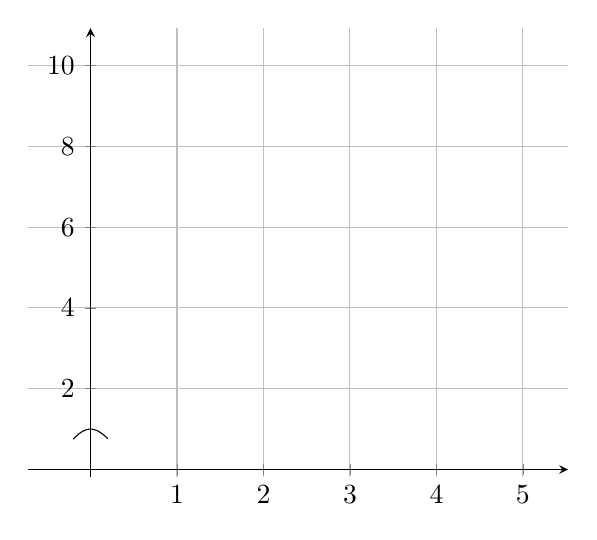
\begin{tikzpicture}
\begin{axis}[grid=both,
          xmax=5,ymax=10,
          axis lines=middle,
          restrict y to domain=-7:7,
          enlargelimits]
\addplot[domain=-0.2:0.2,samples=100]{pow(2,-10*x^2)+x^3};
\end{axis}
\end{tikzpicture}
\end{figure}

Next consider that with a value~$y$ replaced with an infinitely small interval like $[y-\epsilon;y+\epsilon]$:
\begin{figure}[H]
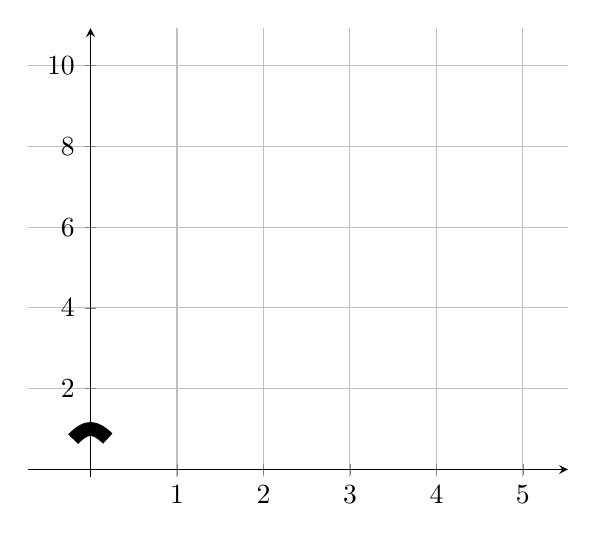
\begin{tikzpicture}
\begin{axis}[grid=both,
          xmax=5,ymax=10,
          axis lines=middle,
          restrict y to domain=-7:7,
          enlargelimits]
\addplot[domain=-0.2:0.2,samples=100,
          line width=5pt]{pow(2,-10*x^2)+x^3};
\end{axis}
\end{tikzpicture}
\end{figure}

Now we have ``an infinitely thin and short strip''. In fact, it is the same as an ``infinitely small rectangle'' (Why? So infinitely small behave, it can be counter-intuitive, but if we consider the above meditations formally, we could get this result):
\begin{figure}[H]
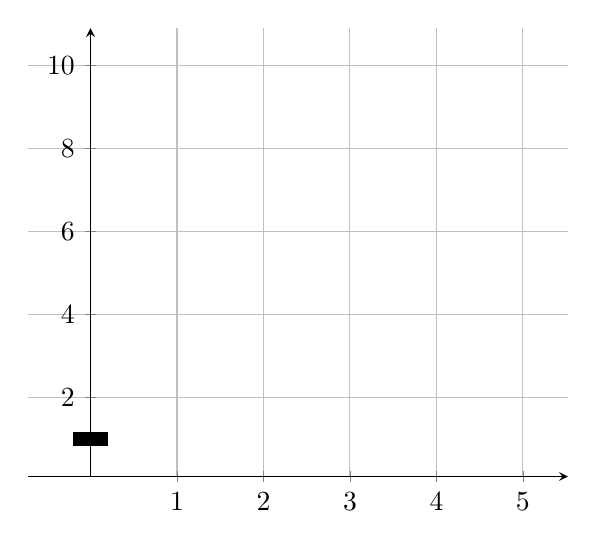
\begin{tikzpicture}
\begin{axis}[grid=both,
          xmax=5,ymax=10,
          axis lines=middle,
          restrict y to domain=-7:7,
          enlargelimits]
\addplot[domain=-0.2:0.2,samples=100,
          line width=5pt]{pow(2,-10)+1};
\end{axis}
\end{tikzpicture}
\end{figure}

This infinitely small rectangle's $y$~position uniquely characterizes the limit of our function (in our example at~$x\to 0$).

If we consider the set of all rectangles we obtain by shifting this rectangle by adding an arbitrary number to~$x$, we get
\begin{figure}[H]
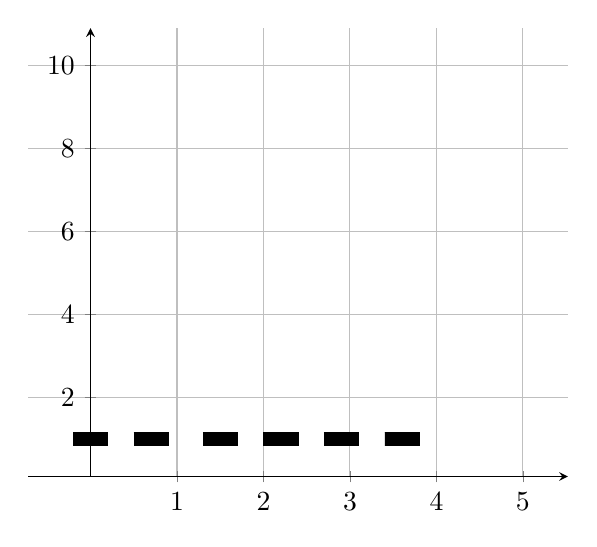
\begin{tikzpicture}
\begin{axis}[grid=both,
          xmax=5,ymax=10,
          axis lines=middle,
          restrict y to domain=-7:7,
          enlargelimits]
\addplot[domain=-0.2:0.2,samples=100,
          line width=5pt]{pow(2,-10)+1};
\addplot[domain=0.5:0.9,samples=100,
          line width=5pt]{pow(2,-10)+1};
\addplot[domain=1.3:1.7,samples=100,
          line width=5pt]{pow(2,-10)+1};
\addplot[domain=2.0:2.4,samples=100,
          line width=5pt]{pow(2,-10)+1};
\addplot[domain=2.7:3.1,samples=100,
          line width=5pt]{pow(2,-10)+1};
\addplot[domain=3.4:3.8,samples=100,
          line width=5pt]{pow(2,-10)+1};
\end{axis}
\end{tikzpicture}
\end{figure}
Such sets one-to-one corresponds to the value of the limit of our function (at $x\to 0$): Knowing such the set, we can calculate the limit (take its arbitrary element and get its so to say $y$-limit point) and knowing the limit value~($y$), we could write down the definition of this set.

So we have a formula for \emph{generalized limit}:
\[ \lim_{x\to a} f(x) =
\{ \nu \circ f|_{\Delta(a)} \circ r \mid r\in G \} \]
where~$G$ is the group of all horizontal shifts of our space~$\mathbb{R}$, $f|_{\Delta(a)}$ is the function~$f$ of which we are taking limit restricted to the infinitely small interval~$\Delta(a)$ around the point~$a$, $\nu\circ{}$~is ``stretching'' our function graph into the infinitely thin ``strip'' by applying a topological operation to it.

What all this (especially ``infinitely small'') means? Read my books ??.

Note that for discontinuous functions elements of our set (our limit is a set) won't be infinitely small ``rectangles'' (as on the pictures), but would ``touch'' more than just one~$y$ value.

The interesting thing here is that we can apply the above formula to \emph{every} function: for example to a discontinuous function, Dirichlet function, unbounded function, unbounded and discontinuous at every point function, etc. In short, the generalized limit is defined for \emph{every} function. We have a definition of limit for every function, not only a continuous function!

And it works not only for real numbers. It would work for example for any function between two topological vector spaces (a vector space with a topology).

Hurrah! Now we can define derivative and integral of \emph{every} function.
\end{document}
